\chapter{OOP 1: Klassen und Objekte}
\renewcommand{\chaptertitle}{OOP 1: Klassen und Objekte}

\lehead[]{\normalfont\sffamily\hspace*{-2.00cm}\textcolor{white}{\colorbox{lightblue}{\makebox[1.60cm][r]{\thechapter}}}\hspace{0.17cm}\textcolor{lightblue}{\chaptertitle}}
\rohead[]{\textcolor{lightblue}{\chaptertitle}\normalfont\sffamily\hspace*{0.17cm}\textcolor{white}{\colorbox{lightblue}{\makebox[1.60cm][l]{\thechapter}}}\hspace{-2.00cm}}
%\chead[]{}
\rehead[]{\textcolor{lightblue}{AvHG, Inf, My}}
\lohead[]{\textcolor{lightblue}{AvHG, Inf, My}}

\lstset{style=myJava}

\label{ch:KlassenUndObjekte}

Eine \emph{Klasse} bezeichnet eine Gruppe gleichartiger \emph{Objekte}.

Beispiele:

\bgroup
\def\arraystretch{1.2}
\begin{tabular}{|l|l|}
\hline
\textbf{Klasse} & \textbf{Objekte der Klasse} \\ \hline
Sportart & Handball, Badminton, Rudern, Leichtathletik, Boxen \\ \hline
Baum & Erle, Birke, Kastanie, Pappel, Buche \\ \hline
Bundespräsident & Theodor Heuss, Heinrich Lübke, Richard von Weizsäcker,
Johannes Rau \\ \hline
\end{tabular}
\egroup

Bis zu diesem Zeitpunkt habt im Informatik-Unterricht von mir zwar ab und zu Begriffe 
wie \emph{Klasse}, \emph{Objekt} oder auch \emph{Konstruktor} zu hören bekommen - sie 
wurden allerdings noch nicht erklärt.

Ich konnte die Begriffe nicht komplett vermeiden, weil die Programmiersprache Java
zu den sogenannten \emph{objektorientierten Programmiersprachen} gehört und die entsprechenden
Konzepte zwangsläufig bei ihrer Verwendung eine Rolle spielen. So findet sich in jedem unserer
Java-Programme direkt oder sehr nah am Anfang der Datei einer Zeile wie etwa

\begin{lstlisting}
public class Smiley {
\end{lstlisting}

Und in einer Zeile wie

\begin{lstlisting}
Color braun = new Color(139, 69, 19);
\end{lstlisting}

spielen bereits alle drei oben gannten Begriffe eine Rolle:

\lstinline|Color| zu Beginn der Zeile steht für einen Datentyp - auch \emph{Klasse} genannt!

\lstinline|braun| ist der von uns gewählte Name des Objekts. Dieses \emph{Objekt} ist von Datentyp
\lstinline|Color|.

Und schließlich wird noch der (gleichnamige) \emph{Konstruktor} \lstinline|Color()| dieser Klasse 
gebraucht um das neue Objekt tatsächlich zu erzeugen.

Erklärt sind die Begriffe Klasse und Objekt damit allerdings immer noch nicht richtig.

Um dies zu ändern schauen wir noch einmal zurück auf die Art und Weise, wie wir bisher unsere
Programme geschrieben haben.

Beispielsweise die Aufgabe 1 aus dem vorangegangenen Kapitel. Dort sollte ein Wald, bestehend aus
vielen Bäumen erstellt werden. Damit nicht jeder Baum einzeln programmiert werden musste, solltet ihr
zunächst eine Methode \lstinline|baum()| erstellen, die jeweils einen Baum an einer frei zu wählenden
x- und y-Position auf dem Bildschirm zeichnen konnte.

Zur Vorbereitung erstellt ihr nun bitte in eurem eigenen Java-Projekt ein neues Package \lstinline|klassenUndObjekte| 
und inner halb dieses Packages ein weiteres Package \lstinline|hundNichtObjektorientiert|. Dort hinein kopiert ihr
aus dem Ordner \lstinline|10_Java_Klassen/HundOhneObjektorientierung| die Datei \lstinline|HundAnwendung.java|

Analog zur Methode \lstinline|baum()| biete ich euch jetzt in der Klasse \lstinline|HundAnwendung| eine Methode 
\lstinline|hundZeichnen()| an, die einen Hund auf den Bildschirm zeichnet:

\begin{lstlisting}
public void hundZeichnen(Graphics g, int x, int y, Color farbe, ...) {
æ   ...
æ}
\end{lstlisting}

Lasst euch nicht durch die lange Parameterliste der Methode und auch nicht durch die im Vergleich zum
Baum erheblich komplexere Programmierung der Methode irritieren. Das tut nichts zur Sache.

Anders als bei den Bäumen, sollen sich die Hunde nicht nur in ihrer x- und y-Position von einander 
unterscheiden können. Sie sollen auch unterscheidliche Farebn und Geschwindigkeiten haben (die Hunde können 
über den Bildschirm laufen). Im Programmbeispiel soll es zwei Hunde geben, die Bobby und Charlie heißen sollen:

\begin{lstlisting}
æ// Erster Hund: Bobby
æbobbyX = 0;
bobbyY = 0;
bobbyFarbe = Color.RED;
bobbyGeschwindigkeit = 2;

æ// Zweiter Hund: Charlie
æcharlieX = 200;
charlieY = 100;
charlieFarbe = Color.GREEN;
charlieGeschwindigkeit = 5;
\end{lstlisting}

In der \lstinline|myPaint()| Methode werden die Hunde dann gezeichnet:

\begin{lstlisting} 
public void myPaint(Graphics g) {
æ  // wird aufgerufen, wenn das Fenster neu gezeichnet wird
æ  zaehler++;
		
  if (zaehler % 2 == 0) {
    hundZeichnen(g, bobbyX, bobbyY, bobbyFarbe, true, false);
  } else {
    hundZeichnen(g, bobbyX, bobbyY, bobbyFarbe, false, false);
  }
  bobbyX += bobbyGeschwindigkeit;
  if (bobbyX > 500) {
    bobbyX = -60;
  }

  if (zaehler % 2 == 0) {
    hundZeichnen(g, charlieX, charlieY, charlieFarbe, true, true);
  } else {
    hundZeichnen(g, charlieX, charlieY, charlieFarbe, false, true);
  }
  charlieX += charlieGeschwindigkeit;
  if (charlieX > 500) {
    charlieX = -60;
  }
}
\end{lstlisting}

Auch hier solltet ihr euch durch die vergleichbar hohe Komplexität, die durch die
Animation der Hunde auf dem Bildschirm entsteht nicht abgschrecken lassen. Im Kern
funktioniert das hier genauso, wie das Zeichnen des Waldes mit Hilfe der Methode 
\lstinline|baum()|. Die Methode \lstinline|hundZeichnen()| wird dabei mit den
passenden Werten (Parametern) für die beiden Hunde aufgerufen. Ihr könnt das Programm
bei euch ausführen und werdet sehen, dass es funktioniert.

\begin{center}
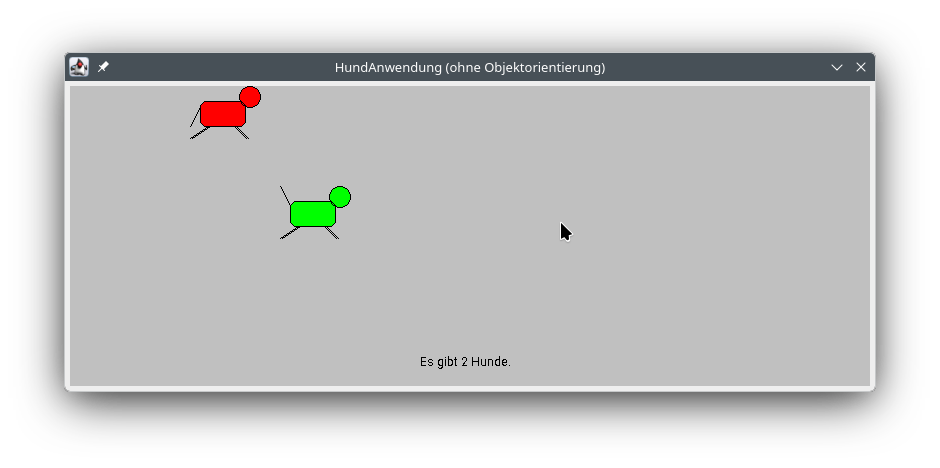
\includegraphics[width=0.6\textwidth]{./inf/SEKII/10_Java_Klassen/HundAnwendung.png}
\end{center}

Schöne ist das allerdings nicht. Bereits jetzt -- mit nur zwei verschiedenen Hunden -- 
ist das Programm nur noch schwer zu lesen! Stellt euch vor, es wären fünf Hunde!

Wie viel schöner wäre es doch, wenn unser Programm so aussehen könnte:

\begin{lstlisting} 
public HundAnwendung(final String title) {
  super(WIDTH, HEIGHT, BACKGROUND, FOREGROUND, title);
æ  // eigene Initialisierung
æ  bobby = new Hund(Color.RED, false);
  charlie = new Hund(200, 100, Color.GREEN);
  maja = new Hund(this);
  Timer timer = new Timer(100, this);
  timer.start();
}

@Override
public void myPaint(Graphics g) {
æ  // wird aufgerufen, wenn das Fenster neu gezeichnet wird
æ		
  maja.zeichnen(g);
		
  bobby.zeichnen(g);
  bobby.bewegen(this, 2);
		
  charlie.zeichnen(g);
  charlie.bewegen(this, 5);
		
  g.drawString("Es gibt " + Hund.getAnzahlHunde() + " Hunde.", 350, 280);
}
\end{lstlisting}

Willkommen in der Objektorientierung!

Hier sind es jetzt drei Hunde (die Hunde Bobby und Charlie verhalten sich exakt so, 
wie in unserem ersten Hunde-Beispiel).

Aber wo ist die ganze Komplexität geblieben, die wir zuvor noch in den Methoden 
\lstinline|hundZeichnen()| und \lstinline|myPaint()| hatten?

Die Komlexität wurde nicht weggezaubert, sondern ausgelagert! Und zwar in eine eigene
Klasse! Das Konzept der objektorientierten Programmierung sieht vor, gleichartige Dinge 
(wie etwa Hunde) in eigenen Klassen zu beschreiben. Es gibt dann eine Aufgabenteilung
zwischen der \emph{Anwendungsklasse} (das ist dass, was ihr bisher immer programmiert 
habt) und der \emph{Fachklasse}.

Die Anwendungslasse ist das Java-Programm, welches sich starten lässt und dann etwas tut 
(beispielsweise einen Wald zeichnet oder animierte Hunde über den Bildschirm laufen lässt).
Anwendungsklassen erstellt ihr bis auf Weiteres immer mit Hilfe des \lstinline|HJFrame|-Templates.
In den Fachklassen hingegen, wird \glqq nur\grqq\ beschrieben, wie gleichartige Dinge 
(beispielsweise Hunde) funktionieren. Genauer: welche Eigenschaften sie haben und was man mit
ihnen tun kann.

Eigenschaften (in der Fachsprache der Objektorientierung auch \emph{Attribute} gennant)
sind nichts anderes als die globalen Variablen der Klasse. Also etwa

\begin{lstlisting}
public class Hund {
  æ// ATTRIBUTE DER KLASSE:
  // Mit Hilfe der globalen Variablen werden die Eigenschaften von Objekten der Klasse 
  // beschrieben.
æ	
  private Color farbe = Color.GRAY;
  private boolean freutSich = false;
  private boolean springend = false;
  æ// Linke obere Ecke des Hundes:
æ  private int x = 0;
  private int y = 0;
æ    .
    .
    .
\end{lstlisting}

Was man mit den Objekten der Fachklasse tun kann, wird durch die \emph{Methoden} der Klasse
beschrieben. Beispielsweise die Methoden \lstinline|zeichnen()| und \lstinline|bewegen()| in der
Klasse Hund.

Wichtig zu verstehen ist, dass die Fachklasse selber nichts tut und nicht als Programm gestartet
werden kann!

Aber durch die Fachklasse wird ein neuer Datentyp (Klasse) definiert mitsamt der Operatoren/Funktionen
(Methoden!), die auf Objekte dieser Klasse angewendet werden können.

In einer Anwendungsklasse können dann Objekte der Fachklasse deklariert und erzeugt werden.
Dabei ist die Deklaration für sich tatsächlich nichts anderes als die Vereinbarung, dass ein bestimmter
Variablenname (Objekt) zu einem bestimmten Datentyp (Klasse) gehört:

\begin{lstlisting}
Hund bobby;
\end{lstlisting}

Diese Deklaration ist nötig, damit das Java-Programm weiß, dass mit bobby ein Hund gemeint ist.
Aber die Deklaration alleine reicht noch nicht! Bevor das so deklarierte Hund-Objektz benutzt werden
kann, muss es erst erzeugt werden! 

Und dazu braucht man einen Konstruktor der entsprechenden Klasse. Konstruktoren haben die Aufgabe
bei der Erzeugung der Objekte dafür zu soregen, dass die Attribute des neuen Objekts mit (hoffentlich 
passenden) Startwerten belegt werden: Konstruktoren haben immer exakt den selben Namen wie die Klasse.
Einschließlich der Groß- und Kleinschreibung! Den Konstruktor benutzt man immer zusammen mit dem
Schlüsselwort \lstinline|new|:

\begin{lstlisting}
Hund charlie;
charlie = new Hund(200, 100, Color.GREEN);
\end{lstlisting} 

Deklaration und Objekterzeugung (die Objekterzeugung wird oft als Initialisierung bezeichnet), können
auch in einem Schritt erfolgen

\begin{lstlisting}
Hund charlie = new Hund(200, 100, Color.GREEN);
\end{lstlisting} 

Auch der (es kann auch mehrere geben) Konstruktor wird in der Fachklasse erstellt.


\section{Darstellung einer Klasse mit der Modellierungssprache UML}

Beispiel: Darstellung der Klasse \myClass{Auto}

\begin{center}
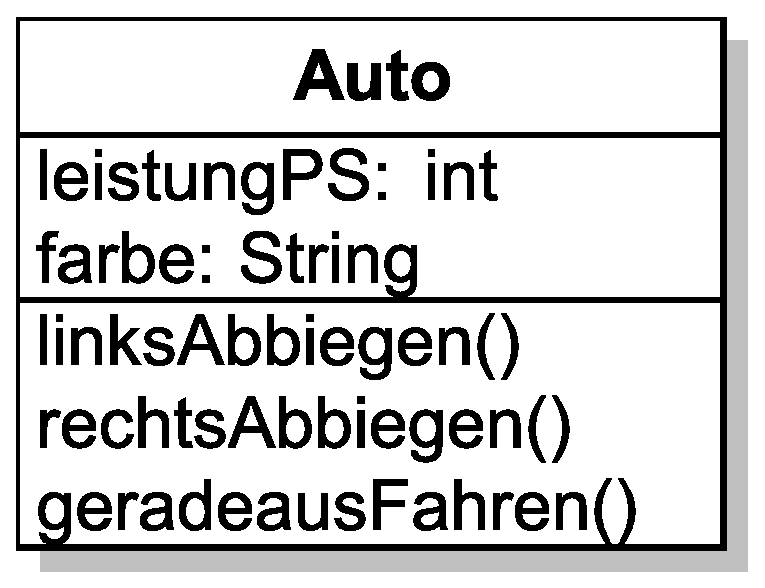
\includegraphics[width=0.2\textwidth]{./inf/SEKII/10_Java_Klassen/Auto.eps}
\end{center}

Das Diagramm einer Klasse ist in drei Abschnitte geteilt. In den obersten
Abschnitt wird der Name der Klasse geschrieben.

In den mittleren Abschnitt trägt man die Eigenschaften der Klasse ein, die für
das Programm, das generiert werden soll, von Bedeutung sind. Die Eigenschaften
bezeichnet man als Attribute. Wenn man die Klasse programmiert, wird für jedes
Attribut eine Variable angelegt. Der Datentyp der Variablen steht durch einen
Doppelpunkt getrennt hinter dem Namen des Attributs.

In den unteren Abschnitt schreibt man die Methoden, die auf die Objekte der
Klasse angewendet werden können.

In der Programmiersprache Java beschreibt eine Klasse das gemeinsame Schema für
alle ihre Objekte. Der Code wird nur einmal programmiert und automatisch auf
jedes Objekt angewendet, das zu der Klasse gehört.


\section{Beispiel: Klasse Hund}

\begin{minipage}{0.5\textwidth}
\begin{center}
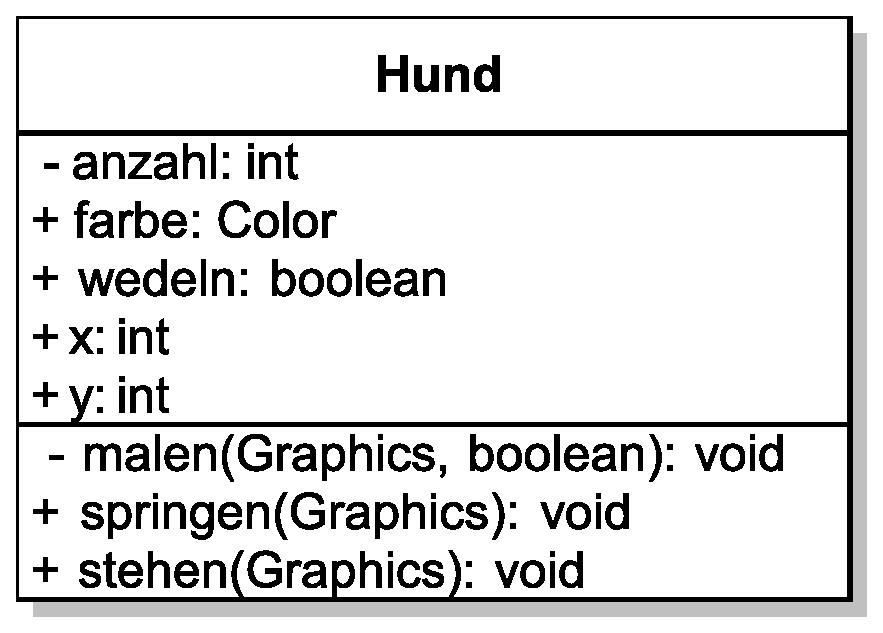
\includegraphics[width=0.66\textwidth]{./inf/SEKII/10_Java_Klassen/HundVorversion.eps}
\end{center}
\end{minipage}
\begin{minipage}{0.5\textwidth}
\subsubsection{Sichtbarkeit}

\lstinline|private| (-) : Variable/Methode kann
nicht von anderer Klasse aufgerufen
werden.

\lstinline|public| (+) : Variable/Methode kann
von jeder anderen Klasse aufgerufen
werden.
\end{minipage}

\subsection{Eine erste Version der Klasse Hund}

(Datei \myFile{HundVorversion.java} im Kurs-Repository)

\begin{lstlisting}
import java.awt.*;

public class Hund {
  public Color farbe = Color.LIGHT_GRAY;
  public boolean wedeln = false;
  public int x = 0;       æ// x- und y-Koordinate der
æ  public int y = 0;       æ// linken oberen Ecke
  // Klassenvariable: zählt die Anzahl aller Hunde - aber wann???
æ  static private int anzahl = 0;

  public void stehen(Graphics g) {     æ// malt den Hund stehend
æ    malen(g, true);
  }

  public void springen(Graphics g) {   æ// malt den Hund springend
æ    malen(g, false);
  }
  
  æ// "interne" Programmierung: malen() ist aus anderen Klassen heraus nicht sichtbar!
æ  private void malen(Graphics g, boolean stehen) {
    Color c = g.getColor();
    if (wedeln) {
      g.drawLine(x+0,y+0,x+10,y+20);
    } else {
      g.drawLine(x+0,y+40,x+10, y+20);
    }
    if (stehen) {
      g.drawLine(x+18, y+40, x+18, y+60);
      g.drawLine(x+20, y+40, x+20, y+60);
      g.drawLine(x+44, y+40, x+44, y+60);
      g.drawLine(x+46, y+40, x+46, y+60);
    } else {
      g.drawLine(x+18, y+40, x+0, y+52);
      g.drawLine(x+20, y+40, x+2, y+52);
      g.drawLine(x+44, y+40, x+56, y+52);
      g.drawLine(x+46, y+40, x+58, y+52);
    }
    g.setColor(farbe);
    g.fillRoundRect(x+10, y+15, 45, 25, 12, 12);
    g.fillOval(x+49,y+0,21,21);
    g.setColor(c);
    g.drawRoundRect(x+10, y+15, 45, 25, 12, 12);
    g.drawOval(x+49,y+0,21,21);
  }
}
\end{lstlisting}


\subsubsection{Was bedeutet static?}

Alle normalen (nicht \lstinline|static|) Variablen und Methoden beziehen sich
immer auf ein spezielles Objekt, dessen Namen man angeben muss.

\lstinline|static| Variable: Es gibt die Variable nur einmal pro Klasse.

\lstinline|static| Methode: Die Methode bezieht sich nicht auf ein einzelnes
Objekt und darf keine Objekt-Variablen verwenden.


Um Objekte der Klasse \myClass{Hund} in einem eigenen Programm zu nutzen würde
man jetzt wie folgt vorgehen. Zunächst würde man eine Variable vom Typ \myClass{Hund}
deklarieren:

\begin{lstlisting}
Hund felix;
\end{lstlisting}

Anschließend könnte man ein entsprechendes \myClass{Hund}-Objekt erzeugen:

\begin{lstlisting}
felix = new Hund();
\end{lstlisting}

Dazu wurde der sogenannte \emph{Konstruktor} der Klasse mit dem
\lstinline|new|-Operator aufgerufen. Ein Konstruktor hätte in der Klasse
\myClass{Hund} programmiert werden können. Aber in der ersten Version der Klasse
\myClass{Hund} ist davon nichts zu sehen.

Tatsächlich \emph{muss} man keinen Konstruktor programmieren. In diesem Fall
gibt es immer einen parameterlosen Konstruktor, der ein neues Objekt der Klasse
erzeugt. Dabei werden alle Objektvariablen so initialisiert, wie es in der
Klasse vorgegeben ist.

Das Hund-Objekt \lstinline|felix| hätte somit zu Beginn folgende Attributwerte:

\begin{tabular}{ll}
\lstinline|farbe| & \lstinline|Color.LIGHT_GRAY| \\
\lstinline|wedeln| \hspace{5mm} & \lstinline|false| \\
\lstinline|x| & \lstinline|0| \\
\lstinline|y| & \lstinline|0| \\
\end{tabular}

Da diese Attribute alle als \lstinline|public| deklariert wurden, lassen sich
diese Werte nun aus der Anwendungsklasse heraus problemlos ändern:

\begin{lstlisting}
felix.x = 100;
felix.y = 250;
felix.farbe = Color.BLACK;
felix.wedeln = true;
\end{lstlisting}

Um unser Hund-Objekt nun im Anwendungsprogramm auch sehen zu können, müssen wir
noch eine der beiden Methoden \lstinline|springen()| oder \lstinline|stehen()|
benutzen:

\begin{lstlisting}
felix.stehen(g);
\end{lstlisting}

Der \myClass{Graphics}-Kontext, den wir in \lstinline|myPaint()| automatisch
haben, ist der benötigte Parameter \lstinline|g|. Die Methoden zum Zeichnen der
Objekte werden also immer innerhalb von \lstinline|myPaint()| aufgerufen (bzw.
in Methoden, die ihrerseits in \lstinline|myPaint()| aufgerufen wurden und den
\myClass{Graphics}-Kontext als Parameter mit übernommen haben).

So weit so gut. Spätestens wenn du eine Hand voll Hunde erzeugt und mit
individuellen Attributwerten ausgestattet hast, wirst du dir jedoch eine
bequemere Methode zum Erzeugen von solchen Objekten wünschen. Wenn dir das nicht
sofort einleuchtet, dann solltest du es ausprobieren!


\subsection{Klasse Hund mit selbstdefinierten Konstruktoren}

Die Lösung besteht darin einen (oder auch mehrere!) Konstruktor in der Klasse
\myClass{Hund} zu programmieren (Datei \myFile{Hund.java} im Kurs-Repository).

Konstruktoren erkennst du daran, dass sie exakt den selben Namen wie die Klasse
tragen (und deshalb im Unterschied zu normalen Methoden auch mit einem
Großbuchstaben beginnen). Außerdem haben sie keinen Rückgabewert. Nicht einmal
das Schlüsselwort \lstinline|void|, welches normalerweise verwendet wird um bei
Methoden anzugeben, dass sie keinen Rückgabewert liefern, wird hier benutzt!

Wenn -- wie in unserem Beispiel hier -- mehrere Konstruktoren programmiert
werden, dann müssen sich diese anhand der Datentypen der Parameterliste
unterscheiden lassen. So kann es beispielsweise nicht zwei verschiedene
Konstruktoren in der selben Klasse geben, die beide als Parameter zwei Integer
Werte erwarten. Anhand der unterschiedlichen Parameterlisten kann der
Java-Compiler dann entscheiden, welcher der vorhandenen Konstruktoren im
konkreten Fall zu benutzen ist.

In unserer Klasse \myClass{Hund} werden vier Konstruktoren definiert. Wenn man
sich die Datentypen der Parameterlisten dieser vier Konstruktoren ansieht,
erkennt man, dass diese eindeutig voneinander unterscheidbar sind:

Liste der Konstruktoren der Klasse \myClass{Hund}:

\begin{tabular}{l}
\lstinline|Hund()| \\
\lstinline|Hund(int, int, Color)| \\
\lstinline|Hund(int, int, boolean)| \\
\lstinline|Hund(Color, boolean)| \\
\end{tabular}

\vspace{1mm}

\begin{lstlisting}
import java.awt.*;

public class Hund {
  public Color farbe = Color.LIGHT_GRAY;
  public boolean wedeln = false;
  public int x = 0;       æ// x- und y-Koordinate der
æ  public int y = 0;       æ// linken oberen Ecke
æ  static private int anzahl = 0; æ// Klassenvariable: Anzahl aller Hunde
æ
  public Hund() {
    wedeln = true;
    anzahl++;
  }

  public Hund(int xPos, int yPos, Color farbe) {
    x = xPos;
    y = yPos;
    this.farbe = farbe;
    wedeln = true;
    anzahl++;
  }

  public Hund(int x, int y, boolean wedeln) {
    this.x = x;
    this.y = y;
    farbe = Color.YELLOW;
    this.wedeln = wedeln;
    anzahl++;
  }

  public Hund(Color f, boolean w) {
    farbe = f;
    wedeln = w;
    anzahl++;
  }

  static public int getAnzahlHunde() {
    return anzahl;
  }

  public void stehen(Graphics g) {      æ// malt den Hund stehend
æ    malen (g, true);
  }
  
  public void springen (Graphics g) {   æ// malt den Hund springend
æ    malen (g, false);
  }

  private void malen (Graphics g, boolean stehen) {
    ...
  }
}
\end{lstlisting}


\section{Objekte erzeugen}

Eine Klasse gibt das Schema für eine Gruppe gleichartiger Objekte vor. Ein
konkret existierendes Objekt bezeichnet man auch als Instanz.

Zum Erzeugen eines Objektes (bzw. einer Instanz) einer Klasse muss man zunächst
eine Variable mit dem Typ der Klasse deklarieren, zum Beispiel:

\begin{lstlisting}
Hund hund1;
\end{lstlisting}

Schema:

\begin{lstlisting}
Klasse variablenname;
\end{lstlisting}

Diese Variable selbst enthält jedoch noch kein Objekt. Die Variable dient dazu
die Speicheradresse abzuspeichern, an der sich die Daten des Objektes im
Hauptspeicher befinden. Solange die Variable noch nicht auf ein Objekt zeigt,
hat sie den Wert \lstinline|null|. \lstinline|null| bedeutet „kein Objekt“.

Das Anlegen eines Objektes und das Abspeichern der Speicheradresse in der
Variablen geschieht zum Beispiel mit folgenden Befehlen:

\begin{lstlisting}
hund1 = new Hund();
hund2 = new Hund(50, 50, Color.YELLOW);
\end{lstlisting}

Schema:

\begin{lstlisting}
Variablename = new Klasse(Parameter);
\end{lstlisting}

Man kann die Deklaration und das Erzeugen des Objektes auch in einem Befehl
zusammen fassen:

\begin{lstlisting}
Hund hund1 = new Hund();
\end{lstlisting}

Wenn es für das Programm nützlich ist, kann man weitere Variablen auf dasselbe
Objekt zeigen lassen:

\begin{lstlisting}
Hund hilfe = hund1;   æ// hilfe zeigt auch auf hund1
\end{lstlisting}

Ein Objekt lebt solange, wie es Variablen gibt, die auf das Objekt verweisen.
Sobald es auf ein Objekt keinen Verweis mehr gibt, wird das Objekt vom System
automatisch vernichtet. Wenn man explizit sagen möchte, dass eine Variable auf
kein Objekt zugreift, so kann man ihr den Wert \lstinline|null| zuweisen:

\begin{lstlisting}
hund1 = null;
\end{lstlisting}


\section{Variablen einer Klasse}

Es gibt drei verschiedene Arten von Variablen, die in dem folgenden Beispiel
verdeutlicht werden:

\begin{lstlisting}
class Beispiel {
  static int klassenVariable;   æ// 1 mal pro Klasse
æ  int objektVariable;           æ// 1 mal pro Objekt
æ
  void methode() {
    int lokaleVariable;         æ// nur innerhalb von methode()
æ  }
}
\end{lstlisting}

\textbf{Klassenvariablen} beziehen sich auf alle Objekte der Klasse und sind
deshalb nur einmal vorhanden. Beispiel: Ein Zähler, der zählt, wie viele Objekte
der Klasse angelegt werden.

\textbf{Objektvariablen} speichern die Daten eines speziellen Objektes, z.B.\
die Farbe eines Hundes. Jedes Objekt besitzt seine eigenen Objektvariablen.

\textbf{Lokale Variablen} werden innerhalb einer Methode deklariert und werden
am Ende der Methode automatisch vom System wieder gelöscht.

Klassen- und Objektvariablen werden vom System automatisch mit \lstinline|0|
bzw.\ \lstinline|false| oder \lstinline|""| (leerer String) initialisiert.
Lokale Variablen dagegen haben zu Beginn einen unbestimmten Wert.


\subsection{Zugriff auf Variablen}

\begin{compactenum}[a)]
\item von außen

Von außen (d.h.\ von einer anderen Klasse aus) greift man auf Klassenvariablen
nach folgendem Schema zu:

\begin{lstlisting}
Klasse.attribut
\end{lstlisting}

Beispiel:

\begin{lstlisting}
Beispiel.klassenVariable = 10;
\end{lstlisting}

Auf eine Objektvariable kann man nur dann zugreifen, wenn man ein Objekt
besitzt. Schema:

\begin{lstlisting}
objekt.attribut
\end{lstlisting}

Beispiel:

\begin{lstlisting}
Beispiel bsp = new Beispiel();
bsp.objektVariable = 5;
\end{lstlisting}

\item innerhalb einer Klasse

Innerhalb einer Klasse kann man auf alle Klassen und Objektvariablen direkt
zugreifen ohne vorher den Klassen- oder Objektnamen anzugeben. Tatsächlich kann
man gar keinen „richtigen“ Objektnamen angeben, da die Klasse ja den Code für
alle Objekte darstellt. Um eine Objektvariable direkt anzusprechen (z.B. um sie
von einer lokalen Variablen mit dem gleichen Namen zu unterscheiden), kann man
das Objekt \lstinline|this| verwenden. \lstinline|this| bezeichnet das aktuelle
Objekt (analog zu dem menschlichen Ausdruck „ich“). In der Klasse Beispiel
könnte beispielsweise stehen:

\begin{lstlisting}
this.objektVariable = 10;
\end{lstlisting}
\end{compactenum}


\section{Methoden}

Methoden, die mit dem Schlüsselwort \lstinline|static| gekennzeichnet sind,
können jederzeit auch ohne Existenz eines Objektes aufgerufen werden. Sie
dürfen jedoch nur Klassenvariablen und lokale Variablen verwenden.

Alle nicht statischen Methoden, werden immer auf ein Objekt der Klasse
angewendet. Mit ihnen kann man die Objektvariablen des aktuellen Objektes
verändern.


\section{Konstruktor}

Der Konstruktor ist eine spezielle Methode, die vom System bei der Erzeugung
eines Objektes mit dem \lstinline|new| Operator aufgerufen wird. Er ist dazu
gedacht, Initialisierungen für das Objekt vorzunehmen (also Anfangswerte für
die Variablen des Objektes zu setzen). Das besondere:

\begin{compactitem}
\item Der Methodenname des Konstruktors ist mit dem Namen der Klasse identisch
\item Der Konstruktor besitzt keinen Rückgabewert (auch nicht
\lstinline|void|!). Aber er kann beliebig viele Parameter besitzen.
\item Der Konstruktor darf niemals explizit aus einer anderen Methode heraus
aufgerufen werden.
\end{compactitem}